\documentclass{article}
\usepackage{amsmath}
\usepackage{amssymb}
\usepackage{enumitem}
\usepackage{algorithm}
\usepackage{listings}
\usepackage{color,xcolor}
\usepackage[T1]{fontenc}
\usepackage{etoolbox}
\usepackage{multicol}
\usepackage{geometry}
\usepackage[colorlinks=true,linkcolor=blue,urlcolor=red,bookmarksopen=true]{hyperref}
\usepackage{tikz, pgfplots, tkz-euclide,calc}
    \usetikzlibrary{patterns,snakes,shapes.arrows,3d,patterns.meta,angles,quotes}
    \geometry{
        total = {160mm, 237mm},
        left = 25mm,
        right = 35mm,
        top = 30mm,
        bottom = 30mm,
      }

\usepackage{tcolorbox}
     \tcbuselibrary{listings,skins}

\newcommand{\enter}{\raisebox{-1.8pt}{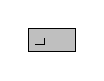
\begin{tikzpicture}[scale=0.3]
    \draw[thin,fill=lightgray] (0,0) rectangle (2,1);
    \draw (0.3,0.3) -- (0.7,0.3)--(0.7,0.6);     
\end{tikzpicture}}}

\definecolor{HIMAmuda}{HTML}{01D1FD}
\definecolor{HIMAtua}{HTML}{02016A}
\definecolor{HIMAabu}{HTML}{CBCBCC}
\definecolor{pgray}{rgb}{0.5,0.5,0.5}
\definecolor{pblue}{rgb}{0.13,0.13,1}
\definecolor{pgreen}{rgb}{0,0.5,0}
\definecolor{pred}{rgb}{0.9,0,0}
\definecolor{pgrey}{rgb}{0.46,0.45,0.48}
\definecolor{pcyan}{HTML}{D4EFFC}
\definecolor{lblue}{HTML}{00AEEF}
\definecolor{input}{HTML}{AAE1FA}
\definecolor{bg}{rgb}{0.95, 0.95, 0.92}
\definecolor{vscode}{HTML}{282A36}
\definecolor{PastelGreen}{HTML}{77DD77}

\newcommand{\inputscan}[1]{\raisebox{0pt}[1pt]{\colorbox{darkgray}{#1}}}

\usepackage{listings}

\lstdefinestyle{Liang}{
language=Java,
showspaces=false,
showtabs=false,
breaklines=true,
showstringspaces=false,
breakatwhitespace=true,
commentstyle=\color{pgray},
keywordstyle=\color{pblue},
stringstyle=\color{pgreen},
basicstyle=\small\ttfamily,
frame=single,
backgroundcolor=\color{pcyan},
escapeinside={(*}{*)},}

\lstdefinestyle{output}{
    language=Java,
    backgroundcolor=\color{vscode},
    basicstyle=\small\ttfamily\color{white},
    frame=none,
    escapeinside={(*}{*)},
    showspaces=false,
    showtabs=false,
    breaklines=true,
    showstringspaces=false,
    breakatwhitespace=true,
    keywordstyle=\color{white},
    }

\lstdefinestyle{standard}{
    language=Java,
    showspaces=false,
    showtabs=false,
    breaklines=true,
    showstringspaces=false,
    breakatwhitespace=true,
    commentstyle=\color{pgray},
    keywordstyle=\color{pblue},
    stringstyle=\color{pgreen},
    basicstyle=\small\ttfamily,
    frame=single,
    backgroundcolor=\color{bg},
    escapeinside={(*}{*)},}
\lstset{style=Liang}

\newtcblisting{RunCode}[1][enhanced,drop shadow]{
    arc=0pt, outer arc=0pt,
    boxsep=1pt,
    boxrule=2pt,
    auto outer arc,
    colback=vscode,
    colframe=bg,
    listing only, 
    listing style=output,
    title=\color{black}Ex. Output,
    #1
    }

\newtcolorbox{hint}[1][]{
    colback=PastelGreen!5!white, 
    colframe=PastelGreen!75!black,
    fonttitle=\bfseries, 
    colbacktitle=PastelGreen!85!black,
    enhanced, 
    attach boxed title to top left={yshift=-2mm}, 
    title=Hint,
    #1
}

\newtcolorbox{req}[1][]{
    colback=lblue!5!white, 
    colframe=lblue!75!black,
    fonttitle=\bfseries, 
    colbacktitle=lblue!85!black,
    enhanced, 
    attach boxed title to top left={yshift=-2mm}, 
    title=Input,
    #1
}

\newtcolorbox{out}[1][]{
    colback=HIMAtua!5!white, 
    colframe=HIMAtua!75!black,
    fonttitle=\bfseries, 
    colbacktitle=HIMAtua!85!black,
    enhanced, 
    attach boxed title to top left={yshift=-2mm}, 
    title=Output,
    before upper=\renewcommand\thempfootnote{\Roman{mpfootnote}},
    #1
}

\renewcommand{\thesubsection}{\arabic{subsection}}
\newcommand{\R}{\mathbb{R}}
\newcommand{\Z}{\mathbb{Z}}

\title{\textbf{Tugas Pertemuan 7}}
\date{
}
\author{Dhanar A \& Fajar A}
\begin{document}

\maketitle

\begin{enumerate}
    %No 1
    \item Pada class Number buatlah static method

    \begin{lstlisting}[style=standard]
    public static boolean perfect(int n)
    \end{lstlisting}
    
    yang menentukan apakah $n$ adalah bilangan sempurna atau tidak

    \begin{hint}
        Bilangan sempurna adalah bilangan dimana jumlah dari seluruh pembagi positif selain dirinya sama dengan dirinya sendiri. \\
        \textbf{Contoh :}
       
        \begin{itemize}
            \item  6 adalah bilangan sempurna\\
            Faktor pembagi positif nya : 1, 2, 3, 6 \\
            Jumlah pembagi positif selain dirinya : $1+2+3=6$

            \item 8 bukanlah bilangan sempurna\\
            Faktor pembagi positif nya : 1, 2, 4, 8 \\
            Jumlah pembagi positif selain dirinya : $1+2+4=7$
        \end{itemize}
    \end{hint}

    \newpage
    %No 2
    \item Pada class Factor buatlah static method 
    \begin{enumerate}
        \item \textbf{gcd}\\
            \begin{lstlisting}[style=standard]
    public static int gcd(int n, int m)
            \end{lstlisting}
            yang menghitung faktor persekutuan terbesar dari m dan n.

        \item \textbf{lcm}\\
            \begin{lstlisting}[style=standard]
    public static long lcm(int n, int m)
            \end{lstlisting}
            yang menghitung kelipatan persekutuan terkecil dari m dan n.
    \end{enumerate}

    \begin{hint}
        Input bisa saja bernilai negatif
    \end{hint}

    
    \newpage
    %No 3
    \item Pada class Circumcircle buatlah static method 
    \begin{enumerate}
        \item radius \\
         \begin{lstlisting}[style=standard]
public static float radius(float ax, float ay, float bx, float by, float cx, float cy)
            \end{lstlisting}
             yang menghitung radius dari lingkaran luar yang dibangun dari titik-titik a, b, c, benar sampai 6 angka di belakang koma.

        \item circumference \\
        \begin{lstlisting}[style=standard]
public static float circumference(float ax, float ay, float bx, float by, float cx, float cy)
            \end{lstlisting}
            yang menghitung keliling dari lingkaran luar yang dibangun dari titik-titik a, b, c, benar sampai 2 angka di belakang koma.

        \item area \\
        \begin{lstlisting}[style=standard]
public static float area(float ax, float ay, float bx, float by, float cx, float cy)
            \end{lstlisting}
            yang menghitung area dari lingkaran luar yang dibangun dari titik-titik a, b, c, benar sampai 2 angka di belakang koma.
    \end{enumerate}

    \begin{hint}
        Cek kondisi kolinear dari titik-titik nya
    \end{hint}
\end{enumerate}

\end{document}
